\documentclass[british, final
              ]{article}

\usepackage[l2tabu,orthodox]{nag}
\usepackage{fixltx2e}
\usepackage{babel}
\usepackage[iso]{isodate}
\usepackage[utf8]{inputenc}
\usepackage[T1]{fontenc}
\usepackage[protrusion=true, expansion=true]{microtype}
\usepackage[strict=true]{csquotes}
\usepackage{xspace}

\usepackage{mathpazo}
\usepackage[scaled=0.95]{helvet}
\usepackage{courier}

\usepackage{fullpage}
\usepackage{hyperref}
\usepackage[missing=0.9.12]{gitinfo}

\usepackage{multicol}
\usepackage{enumitem}

\usepackage{fpmacros}
\usepackage{idrislang}
\usepackage{comment}
\usepackage{graphicx}

\input{conf.ltx}
\input{library.ltx}

\newcommand{\version}{\gitVtagn}
\newcommand{\effects}{\texttt{neweffects}}

\title{Programming and Reasoning with Side-Effects in \Idris{}}
\author{Edwin Brady}
\date{\origdate\today}

\begin{document}

\maketitle
\tableofcontents
\newpage

\section{Introduction}

Pure functional languages with dependent types such as \Idris{}
(\url{http://idris-lang.org/})
support reasoning about programs directly in the type system, promising that we
can \emph{know} a program will run correctly (i.e. according to the
specification in its type) simply because it compiles. Realistically, though,
things are not so simple: programs have to interact with the outside world,
with user input, input from a network, mutable state, and so on. In this
tutorial I will introduce the \effects{} library, which is included with
the \Idris{} distribution and supports programming and reasoning with
side-effecting programs, supporting mutable state, interaction with the
outside world, exceptions, and verified resource management.

This tutorial assumes familiarity with pure programming in \Idris{}, as
described in Sections 1--6 of the main
tutorial~\cite{idris-tutorial}\footnote{You do not, however, need to know what
a monad is. A correctness property of this tutorial is that the word ``monad''
should appear exactly twice, both in this footnote.}. The examples are
tested with \Idris{} version \version{}.

Consider, for example, the following introductory function which illustrates
the kind of properties which can be expressed in the type system:

\begin{code}
vadd : Vect n Int -> Vect n Int -> Vect n Int
vadd []        []        = []
vadd (x :: xs) (y :: ys) = x + y :: vadd xs ys
\end{code}

This function adds corresponding elements in a pair of vectors. The type
guarantees that the vectors will contain only elements of type \texttt{Int},
and that the input lengths and the output length all correspond. A natural
question to ask here, which is typically neglected by introductory tutorials,
is ``How do I turn this into a program?'' That is, given some lists entered
by a user, how do we get into a position to be able to apply the 
\texttt{vadd} function? Before doing so, we will have to:

\begin{itemize}
\item Read user input, either from the keyboard, a file, or some other input device.
\item Check that the user inputs are valid, i.e. contain only \texttt{Int}s and
are the same length, and report an error if not.
\item Write output
\end{itemize}

The complete program will include side-effects for I/O and error handling,
before we can get to the pure core functionality. In this tutorial, we will
see how \Idris{} supports side-effects. Furthermore, we will see how we can 
use the dependent type system to \emph{reason} about stateful and
side-effecting programs. We will return to this specific example later.

\subsection{Hello world}

To give an idea of how programs with effects look in \Idris{}, here is the
ubiquitus ``Hello world'' program, written using the \effects{} library:

\begin{code}
module Main
  
import Effect.StdIO
  
hello : { [STDIO] } Eff IO ()
hello = putStrLn "Hello world!"
  
main : IO ()
main = run hello
\end{code}

\noindent
As usual, the entry point is \texttt{main}. All \texttt{main} has to do is
invoke the \texttt{hello} function which supports the \texttt{STDIO} effect
for console I/O, runs in the \texttt{IO} context, and returns the unit
value. The details of the \texttt{Eff} type will be presented in the
remainder of this tutorial.

To compile and run this program, \Idris{} needs to be told to include the
\effects{} package, using the \texttt{-p} \effects{} flag (this flag
is required for all examples in this tutorial):

%FIXME: \effects{} macro didn't work here, make sure to update it...
\begin{code}
$ idris hello.idr -o hello -p effects
$ ./hello
Hello world!
\end{code}

\subsection{Outline}

The tutorial is structured as follows: first, in Section \ref{sect:state},
we will discuss state management, describing why it is important and introducing
the \effects{} library to show how it can be used to manage state. This section
also gives an overview of the syntax of effectful programs. Section
\ref{sect:simpleff} then introduces a number of other effects a program may
have: I/O; Exceptions; Random Numbers; and Non-determinism, giving examples
for each, and an extended example combining several effects in one complete
program. Section \ref{sect:depeff} introduces \emph{dependent} effects, showing
how states and resources can be managed in types. Section \ref{sect:impleff}
shows how new effects can be implemented. Section \ref{sect:hangman}
gives an extended example showing how to implement a ``mystery word'' guessing
game, using effects to describe the rules of the game and ensure they are
implemented accurately. References to further reading are given in
Section \ref{sect:further}.


\section{State}

Many programs, even pure programs, can benefit from locally mutable state.
For example, consider a program which tags binary tree nodes with a counter,
by an inorder traversal (i.e. counting depth first, left to right). This
would perform something like the following:

\begin{center}
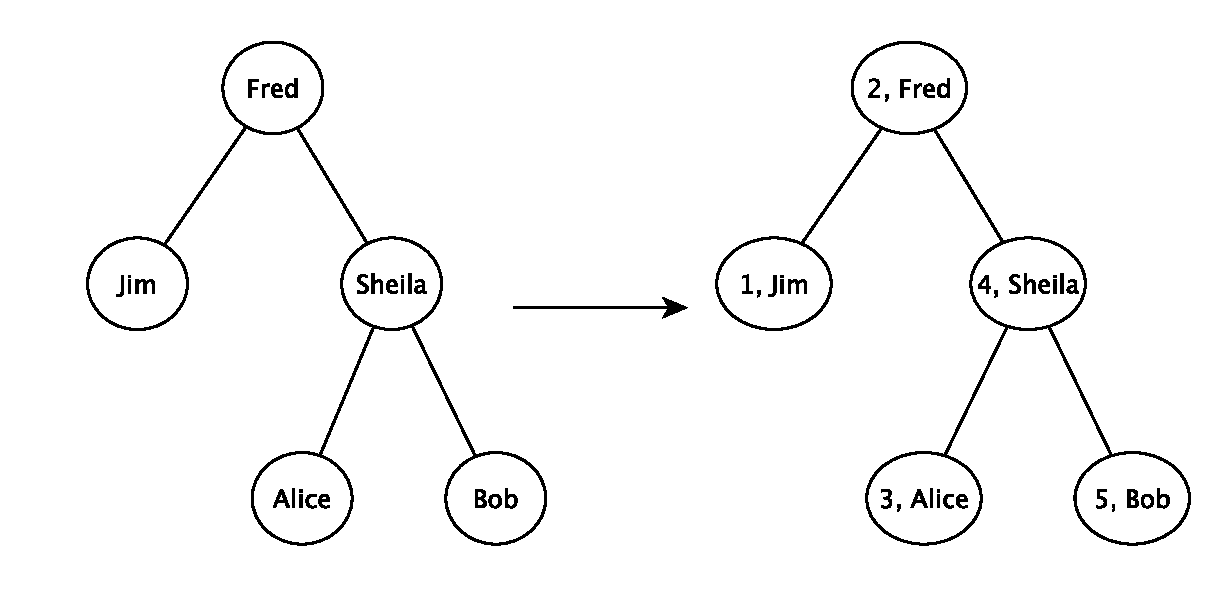
\includegraphics[width=12cm]{content/treelabel.pdf}
\end{center}

\noindent
We can describe binary trees with the following data type \texttt{BTree}
and \texttt{testTree} to represent the example input above:

\begin{code}
data BTree a = Leaf
             | Node (BTree a) a (BTree a)

testTree : BTree String
testTree = Node (Node Leaf "Jim" Leaf)
                "Fred"
                (Node (Node Leaf "Alice" Leaf)
                      "Sheila"
                      (Node Leaf "Bob" Leaf))
\end{code}

\noindent
Then our function to implement tagging, beginning to tag with a specific
value \texttt{i}, has the following type:

\begin{code}
treeTag : (i : Int) -> BTree a -> BTree (Int, a)
\end{code}

\subsubsection*{First attempt}

Na\"{i}vely, we can implement \texttt{treeTag} by implementing a helper
function which propagates a counter, returning the result of the count for
each subtree:

\begin{code}
treeTagAux : (i : Int) -> BTree a -> (Int, BTree (Int, a))
treeTagAux i Leaf = (i, Leaf)
treeTagAux i (Node l x r)
       = let (i', l') = treeTagAux i l in
         let x' = (i', x) in
         let (i'', r') = treeTagAux (i' + 1) r in
             (i'', Node l' x' r')
  
treeTag : (i : Int) -> BTree a -> BTree (Int, a)
treeTag i x = snd (treeTagAux i x)
\end{code}

\noindent
This gives the expected result when run at the \Idris{} REPL prompt:

\begin{code}
*TreeTag> treeTag 1 testTree 
Node (Node Leaf (1, "Jim") Leaf)
     (2, "Fred")
     (Node (Node Leaf (3, "Alice") Leaf)
           (4, "Sheila")
           (Node Leaf (5, "Bob") Leaf)) : BTree (Int, String)
\end{code}

\noindent
This works as required, but there are several problems when we try to scale
this to larger programs. It is error prone, because we need to ensure that
state is propagated correctly to the recursive calls (i.e. passing the
appropriate \texttt{i} or \texttt{i'}). It is hard to read, because the
functional details are obscured by the state propagation. Perhaps most
importantly, there is a common programming pattern here which should be
abstracted but instead has been implemented by hand. There is local mutable
state (the counter) which we have had to make explicit.

\subsection{Introducing \effects{}}

\Idris{} provides a library, \effects{}~\cite{brady-icfp2013}, which captures
this pattern and many others involving effectful computation\footnote{The
earlier paper~\cite{brady-icfp2013} describes the essential implementation
details, although the library presented there is an earlier version which is
less powerful than that presented in this tutorial.}. An effectful program
\texttt{f} has a type of the following form:

\begin{code}
f : (x1 : a1) -> (x2 : a2) -> ... -> { effs } Eff m t
\end{code}

\noindent
That is, the return type gives the effects that \texttt{f} supports
(\texttt{effs}, of type \texttt{List EFFECT}), 
the \emph{computation context} it runs in (\texttt{m}) and the
type the computation returns \texttt{t}. The computation context can be
any function of type \texttt{Type -> Type}, for example \texttt{id}. So, our
\texttt{treeTagAux} helper could be written with the following type:

\begin{code}
treeTagAux : BTree a -> { [STATE Int] } Eff id (BTree (Int, a))
\end{code}

\noindent
That is, \texttt{treeTagAux} has access to an integer state, because the
list of available effects includes \texttt{STATE Int}. \texttt{STATE} is
declared as follows in the module \texttt{Effect.State} (that is, we must
\texttt{import Effect.State} to be able to use it:

\begin{code}
STATE : Type -> EFFECT
\end{code}

\noindent
That is, it is an effect parameterised by a type (by convention, we write
effects in all capitals).
The \texttt{treeTagAux} function runs in the
identity computation context and
returns a new tree tagged with \texttt{Ints}. It is implemented as
follows:

\begin{code}
treeTagAux Leaf = pure Leaf
treeTagAux (Node l x r)
    = do l' <- treeTagAux l
         i <- get
         put (i + 1)
         r' <- treeTagAux r
         pure (Node l' (i, x) r')
\end{code}

\noindent
There are several remarks to be made about this implementation. Essentially,
it hides the state, which can be accessed using \texttt{get} and updated using
\texttt{put}, but it introduces several new features. Specifically, it uses
\texttt{do}-notation, binding variables with \texttt{<-}, and a
\texttt{pure} function. There is much to be said about these features, but
for our purposes, it suffices to know the following:

\begin{itemize}
\item \texttt{do} blocks allow effectful operations to be sequenced.
\item \texttt{x <- e} binds the result of an effectful operation \texttt{e} to
a variable \texttt{x}. For example, in the above code, \texttt{treeTagAux l}
is an effectful operation returning a pair \texttt{(Int, BTree a)}, so
\texttt{l'} has type \texttt{(Int, BTree a)}.
\item \texttt{pure e} turns a pure value \texttt{e} into the result of
an effectful operation. 
\end{itemize}

\noindent
The \texttt{get} and \texttt{put} functions read and write a state \texttt{t}, 
assuming that the \texttt{STATE t} effect is available. They have the following
types, polymorphic in the state \texttt{t} they manage:

\begin{code}
get :      { [STATE t] } Eff m t
put : t -> { [STATE t] } Eff m () 
\end{code}

\noindent
A program in \texttt{Eff} can call any other function in \texttt{Eff} provided
that the calling function supports at least the effects required by the called
function. In this case, it is valid for \texttt{treeTagAux} to call both
\texttt{get} and \texttt{put} because all three functions support the
\texttt{STATE Int} effect.

To run a program in \texttt{Eff} (that is, to evaluate it in an appropriate
context), we use the \texttt{run} or \texttt{runPure} function. Using 
\texttt{runPure}, which runs an effectful program in the identity context,
we can write the \texttt{treeTag} function as follows, using \texttt{put}
to initialise the state:

\begin{code}
treeTag : (i : Int) -> BTree a -> BTree (Int, a)
treeTag i x = runPure (do put i
                          treeTagAux x)
\end{code}

\noindent
We could also run the program in an impure context, such as \texttt{IO},
by changing the type of \texttt{treeTagAux} to be polymorphic in computation
contexts, and using \texttt{run} instead of \texttt{runPure}:

\begin{code}
treeTagAux : BTree a -> { [STATE Int] } Eff m (BTree (Int, a))
...

treeTag : (i : Int) -> BTree a -> IO (BTree (Int, a))
treeTag i x = run (do put i
                      treeTagAux x)
\end{code}

\noindent
Note that the definition of \texttt{treeTagAux} is exactly as before. All that
has changed is that the type is more generic, and can run in \emph{any}
computation context \texttt{m}. There are no constraints on \texttt{m} other
than that it must have type \texttt{Type -> Type}. For reference, this
complete program (including a \texttt{main} to run it) is shown in
Listing \ref{introprog}.


\begin{code}[float=h,frame=single,caption={Tree tagging}, label=introprog]
module Main

import Effect.State

data BTree a = Leaf
             | Node (BTree a) a (BTree a)

instance Show a => Show (BTree a) where
    show Leaf = "[]"
    show (Node l x r) = "[" ++ show l ++ " "
                            ++ show x ++ " "
                            ++ show r ++ "]"

testTree : BTree String
testTree = Node (Node Leaf "Jim" Leaf)
              "Fred"
              (Node (Node Leaf "Alice" Leaf)
                    "Sheila"
                    (Node Leaf "Bob" Leaf))

treeTagAux : BTree a -> { [STATE Int] } Eff m (BTree (Int, a))
treeTagAux Leaf = pure Leaf
treeTagAux (Node l x r)
  = do l' <- treeTagAux l
       i <- get
       put (i + 1)
       r' <- treeTagAux r
       pure (Node l' (i, x) r')

treeTag : (i : Int) -> BTree a -> BTree (Int, a)
treeTag i x = runPure (do put i
                          treeTagAux x)

main : IO () 
main = print (treeTag 1 testTree) 
\end{code}


\subsection{Effects and Resources}

Each effect is associate with a \emph{resource}, which is initialised before
an effectful program can be run. For example, in the case of \texttt{STATE Int}
the corresponding resource is the integer state itself.
The types of \texttt{runPure} and \texttt{run} show this (slightly
simplified here for illustrative purposes):

\begin{code}
runPure : {env : Env id xs} -> { xs } Eff id a -> a
run : Applicative m => {env : Env m xs} -> { xs } Eff m a -> m a
\end{code}

\noindent
The \texttt{env} argument is implicit, and initialised automatically where
possible using default values given by instances of the following type class:

\begin{code}
class Default a where
    default : a
\end{code}

\noindent
Instances of \texttt{Default} are defined for all primitive types, and many
library types such as \texttt{List}, \texttt{Vect}, \texttt{Maybe}, pairs,
etc. However, where no default value exists for a resource type (for example,
you may want a \texttt{STATE} type for which there is no \texttt{Default}
instance) the resource environment can be given explicitly using one of
the following functions:

\begin{code}
runPureInit : Env id xs -> { xs } Eff id a -> a
runInit : Applicative m => Env m xs -> { xs } Eff m a -> m a
\end{code}

\noindent
To be well-typed, the environment must contain resources corresponding exactly
to the effects in \texttt{xs}.
For example, we could also have implemented \texttt{treeTag} by initialising
the state as follows:

\begin{code}
treeTag : (i : Int) -> BTree a -> BTree (Int, a)
treeTag i x = runPureInit [i] (treeTagAux x)
\end{code}

\subsection{Labelled Effects}

What if we have more than one state, especially more than one state of the
same type? How would \texttt{get} and \texttt{put}
know which state they should be referring to? For example, how could we
extend the tree tagging example such that it additionally counts the number
of leaves in the tree?
%
One possibility would be to change the state so that it captured both of
these values, e.g.:

\begin{code}
treeTagAux : BTree a -> { [STATE (Int, Int)] } Eff m (BTree (Int, a))
\end{code}

\noindent
Doing this, however, ties the two states together throughout (as well as
not indicating which integer is which). It would be nice to be able to
call effectful programs which guaranteed only to access one of the states,
for example. In a larger application, this becomes particularly important.

The \effects{} library therefore allows effects in general to be
\emph{labelled} so that they can be referred to explicitly by a particular
name. This allows multiple effects of the same type to be included. We can
count leaves and update the tag separately, by labelling them as follows:

\begin{code}
treeTagAux : BTree a -> { ['Tag ::: STATE Int,
                           'Leaves ::: STATE Int] } Eff m (BTree (Int, a))
\end{code}

\noindent
The \texttt{:::} operator allows an arbitrary label to be given to an effect.
This label can be any type---it is simply used to identify an effect uniquely.
Here, we have used a symbol type. In general \texttt{'name} introduces a
new symbol, the only purpose of which is to disambiguate values\footnote{In
practice, \texttt{'name} simply introduces a new empty type}. 

When an effect is labelled, its operations are also labelled using the
\texttt{:-} operator. In this way, we can say explicitly which state we mean
when using \texttt{get} and \texttt{put}. The tree tagging program which also
counts leaves can be written as follows:

\begin{code}
treeTagAux Leaf = do 'Leaves :- update (+1)
                     pure Leaf
treeTagAux (Node l x r)
  = do l' <- treeTagAux l
       i <- 'Tag :- get
       'Tag :- put (i + 1)
       r' <- treeTagAux r
       pure (Node l' (i, x) r')
\end{code}

\noindent
The \texttt{update} function here is a combination of \texttt{get} and \texttt{put},
applying a function to the current state.

\begin{code}
update : (x -> x) -> { [STATE x] } Eff m () 
\end{code}

\noindent
Finally, our top level \texttt{treeTag} function now returns a pair of
the number of leaves, and the new tree. Resources for labelled effects are
intialised using the \texttt{:=} operator (reminisicent of assignment in
an imperative language):

\begin{code}
treeTag : (i : Int) -> BTree a -> (Int, BTree (Int, a))
treeTag i x = runPureInit ['Tag := i, 'Leaves := 0]
                    (do x' <- treeTagAux x
                        leaves <- 'Leaves :- get
                        pure (leaves, x'))
\end{code}

\noindent
To summarise, we have:

\begin{itemize}
\item \texttt{:::} to convert an effect to a labelled effect.
\item \texttt{:-} to convert an effectful operation to a labelled effectful operation.
\item \texttt{:=} to initialise a resource for a labelled effect.
\end{itemize}

\noindent
Or, more formally with their types (slightly simplified to account only for
the situation where available effects are not updated):

\begin{code}
(:::) : lbl -> EFFECT -> EFFECT
(:-)  : (l : lbl) -> { [x] } Eff m a -> { [l ::: x] } Eff m a
(:=)  : (l : lbl) -> res -> LRes l res
\end{code}

\noindent
Here, \texttt{LRes} is simply the resource type associated with a labelled
effect. Note that labels are polymorphic in the label type \texttt{lbl}. 
Hence, a label can be anything---a string, an integer, a type, etc.

\subsection{\texttt{!}-notation}

In many cases, using \texttt{do}-notation can make programs unnecessarily
verbose, particularly in cases where the value
bound is used once, immediately. The following program returns the length of
the \texttt{String} stored int the state, for example:

\begin{code}
stateLength : { [STATE String] } Eff m Nat
stateLength = do x <- get
                 pure (length x)
\end{code}

\noindent
This seems unnecessarily verbose, and it would be nice to program in a more
direct style in these cases. \Idris{} provides \texttt{!}-notation to help
with this. The above program can be written instead as:

\begin{code}
stateLength : { [STATE String] } Eff m Nat
stateLength = pure (length !get)
\end{code}

\noindent
The notation \texttt{!expr} means that the expression \texttt{expr} should
be evaluated and then implicitly bound. Conceptually,
we can think of \texttt{!} as being a prefix function with the following type:

\begin{code}
(!) : { xs } Eff m a -> a
\end{code}

\noindent
Note, however, that it is not really a function, merely syntax! In practice, a
subexpression \texttt{!expr} will lift \texttt{expr} as high as possible within
its current scope, bind it to a fresh name \texttt{x}, and replace
\texttt{!expr} with \texttt{x}. Expressions are lifted depth first, left to
right. In practice, \texttt{!}-notation allows us to program in a more direct
style, while still giving a notational clue as to which expressions are
effectful.

For example, the expression\ldots

\begin{code}
let y = 42 in f !(g !(print y) !x) 
\end{code}

\ldots is lifted to:

\begin{code}
let y = 42 in do y' <- print y
                 x' <- x
                 g' <- f y' x'
                 f g'
\end{code}


\subsection{Syntactic Sugar and \texttt{Eff}}

By now, you may be wondering about the syntax we are using for \texttt{Eff},
because it doesn't look like a normal \Idris{} type! (If not, you may
safely skip this section and return to it later.) In fact, the type of
\texttt{Eff} is the following:

\begin{code}
Eff : (m : Type -> Type) ->
      (x : Type) ->
      List EFFECT -> (x -> List EFFECT) -> Type
\end{code}

\noindent
This is more general than the types we have been writing so far. It is
parameterised over a computation context \texttt{m}, a result type \texttt{x},
as we have already seen, but also a \texttt{List EFFECT} and a function type
\texttt{x -> List EFFECT}.

These additional parameters are the list of \emph{input} effects, and a list
of \emph{output} effects, computed from the result of an effectful operation.
That is: running an effectful program can change the set of effects available!
This is a particularly powerful idea, and we will see its consequences in more
detail later. Some examples of operations which can change the set of available
effects are:

\begin{itemize}
\item Updating a state containing a dependent type (for example adding an
element to a vector).
\item Opening a file for reading is an effect, but whether the file really
\emph{is} open afterwards depends on whether the file was successfully opened.
\item Closing a file means that reading from the file should no longer be
possible.
\end{itemize}

\noindent
While powerful, this can make uses of the \texttt{Eff} type hard to read.
Therefore, the \effects{} library provides syntactic sugar which is translated
such that\ldots

\begin{code}
{ xs } Eff m a 
\end{code}

\ldots is expanded to \ldots

\begin{code}
Eff m a xs (\_ => xs)
\end{code}

\noindent
i.e. the set of effects remains the same on output. This suffices for the
\texttt{STATE} example we have seen so far, and for many useful side-effecting
programs. We could also have written \texttt{treeTagAux} with the expanded
type:

\begin{code}
treeTagAux : BTree a -> 
             Eff m (BTree (Int, a)) [STATE Int] (\x => [STATE Int])
\end{code}

\noindent
Later, we will see programs which update effects:

\begin{code}
{ xs ==> xs' } Eff m a
\end{code}

\ldots which is expanded to \ldots

\begin{code}
Eff m a xs (\_ => xs')
\end{code}

\noindent
i.e. the set of effects is updated to \texttt{xs'} (think of a transition
in a state machine). There is, for example, a version of \texttt{put} which
updates the type of the state:

\begin{code}
putM : y -> { [STATE x] ==> [STATE y] } Eff m () 
\end{code}

\noindent
Also, we have:

\begin{code}
{ {res} xs ==> xs' } Eff m a
\end{code}

\ldots which is expanded to \ldots

\begin{code}
Eff m a xs (\res => xs')
\end{code}

\noindent
i.e. the set of effects is updated according to the result of the operation
\texttt{res}.





\section{Simple Effects}

So far we have seen how to write programs with locally mutable state using the
\texttt{STATE} effect. To recap, we have the definitions in
Listing \ref{eff:state} in a module \texttt{Effect.State}.

\begin{code}[float=h,frame=single,caption={State Effect},label=eff:state]
module Effect.State

STATE : Type -> EFFECT

get    :             { [STATE x] } Eff m x
put    : x ->        { [STATE x] } Eff m () 
putM   : y ->        { [STATE x] ==> [STATE y] } Eff m () 
update : (x -> x) -> { [STATE x] } Eff m () 

instance Handler State m
\end{code}

\noindent
The last line, \texttt{instance Handler State m}, means that the \texttt{STATE}
effect is usable in any computation context \texttt{m}. (The lower case
\texttt{State} is a data type describing the operations which make up the
\texttt{STATE} effect itself---we will go into more
detail about this in Section \ref{sect:impleff}.) 

In this section, we will introduce some other supported effects, allowing
console I/O, exceptions, random number generation and non-deterministic
programming.
For each effect we introduce, we will begin with a summary of the effect,
its supported operations, and the contexts in which it may be used,
like that above for \texttt{STATE}, and go on to
present some simple examples. At the end, we will see some examples of programs
which combine multiple effects.

All of the effects in the library, including those described in this section,
are summarised in Appendix \ref{sect:appendix}.

\subsection{Console I/O}

\begin{code}[float=h,frame=single, caption={Console I/O Effect}, label=eff:stdio]
module Effect.StdIO

STDIO : EFFECT

putChar  : Handler StdIO m => Char ->   { [STDIO] } Eff m ()
putStr   : Handler StdIO m => String -> { [STDIO] } Eff m ()
putStrLn : Handler StdIO m => String -> { [STDIO] } Eff m ()

getStr   : Handler StdIO m =>           { [STDIO] } Eff m String
getChar  : Handler StdIO m =>           { [STDIO] } Eff m Char

instance Handler StdIO IO
instance Handler StdIO (IOExcept a)
\end{code}

\noindent
Console I/O (Listing \ref{eff:stdio})
is supported with the \texttt{STDIO} effect, which allows reading
and writing characters and strings to and from standard input and standard
output. Notice that there is a constraint here on the computation context
\texttt{m}, because it only makes sense to support console I/O operations in
a context where we can perform (or at the very least simulate) console I/O.

\subsubsection*{Examples}

A program which reads the user's name, then says hello, can be written
as follows:

\begin{code}
hello : { [STDIO] } Eff IO ()
hello = do putStr "Name? "
           x <- getStr
           putStrLn ("Hello " ++ trim x ++ "!")
\end{code}

\noindent
We use \texttt{trim} here to remove the trailing newline from the input.
The resource associated with \texttt{STDIO} is simply the empty tuple, which
has a default value \texttt{()}, so we can run this as follows:

\begin{code}
main : IO ()
main = run hello
\end{code}

\noindent
In \texttt{hello} we could also use \texttt{!}-notation instead of \texttt{x <-
getStr}, since we only use the string that is read once:

\begin{code}
hello : { [STDIO] } Eff IO ()
hello = do putStr "Name? "
           putStrLn ("Hello " ++ trim !getStr ++ "!")
\end{code}

\noindent
More interestingly, we can combine multiple effects in one program. For example,
we can loop, counting the number of people we've said hello to:

\begin{code}
hello : { [STATE Int, STDIO] } Eff IO ()
hello = do putStr "Name? "
           putStrLn ("Hello " ++ trim !getStr ++ "!")
           update (n + 1)
           putStrLn ("I've said hello to: " ++ show !get ++ " people")
           hello
\end{code}

\noindent
The list of effects given in \texttt{hello} means that the function can
call \texttt{get} and \texttt{put} on an integer state, and any functions
which read and write from the console. To run this, \texttt{main} does
not need to be changed.

\subsubsection*{Aside: Resource Types}

To find out the resource type of an effect, if necessary (for example if
we want to initialise a resource explicitiy with \texttt{runInit} rather than
using a default value with \texttt{run})
we can run the \texttt{resourceType} function at the \Idris{} REPL:

\begin{code}
*ConsoleIO> resourceType STDIO
() : Type
*ConsoleIO> resourceType (STATE Int)
Int : Type
\end{code}

\subsection{Exceptions}

Listing \ref{eff:exception} gives the definition of the \texttt{EXCEPTION}
effect, declared in module \texttt{Effect.Exception}. This allows programs
to exit immediately with an error, or errors to be handled more generally.

\begin{code}[float=h,frame=single,label=eff:exception,caption={Exception Effect}]
module Effect.Exception

EXCEPTION : Type -> EFFECT

raise : a -> { [EXCEPTION a ] } Eff m b 

instance           Handler (Exception a) Maybe
instance           Handler (Exception a) List
instance           Handler (Exception a) (Either a)
instance           Handler (Exception a) (IOExcept a)
instance Show a => Handler (Exception a) IO
\end{code}

\subsubsection*{Example}

Suppose we have a \texttt{String} which is expected to represent an integer in
the range \texttt{0} to \texttt{n}. We can write a function \texttt{parseNumber}
which returns an \texttt{Int} if parsing the string returns a number in the
appropriate range, or throws an exception otherwise. Exceptions are
paramaterised by an error type:

\begin{code}
data Err = NotANumber | OutOfRange

parseNumber : Int -> String -> { [EXCEPTION Err] } Eff m Int
parseNumber num str
   = if all isDigit (unpack str)
        then let x = cast str in
             if (x >=0 && x <= num)
                then pure x
                else raise OutOfRange
        else raise NotANumber
\end{code}

\noindent
Programs which support the \texttt{EXCEPTION} effect can be run in any
context which has some way of throwing errors, for example, we can run
\texttt{parseNumber} in the \texttt{Either Err} context. It returns
a value of the form \texttt{Right x} if successful:

\begin{code}
*Exception> the (Either Err Int) $ run (parseNumber 42 "20")
Right 20 : Either Err Int
\end{code}

\noindent
Or \texttt{Left e} on failure, carrying the appropriate exception:

\begin{code}
*Exception> the (Either Err Int) $ run (parseNumber 42 "50")
Left OutOfRange : Either Err Int

*Exception> the (Either Err Int) $ run (parseNumber 42 "twenty")
Left NotANumber : Either Err Int
\end{code}

\noindent
In fact, we can do a little bit better with \texttt{parseNumber}, and have it
return a \emph{proof} that the integer is in the required range along with
the integer itself. One way to do this is define a type of bounded integers,
\texttt{Bounded}:

\begin{code}
Bounded : Int -> Type
Bounded x = (n : Int ** so (n >= 0 && n <= x))
\end{code}

\noindent
Recall that \texttt{so} is parameterised by a \texttt{Bool}, and only
\texttt{so True} is inhabited. We can use \texttt{choose} to construct such
a value from the result of a dynamic check:

\begin{code}
data so : Bool -> Type = oh : so True

choose : (b : Bool) -> Either (so b) (so (not b))
\end{code}

\noindent
We then write \texttt{parseNumber} using \texttt{choose} rather than
an \texttt{if/then/else} construct, passing the proof it returns on success
as the boundedness proof:

\begin{code}
parseNumber : (x : Int) -> String -> { [EXCEPTION Err] } Eff m (Bounded x)
parseNumber x str
   = if all isDigit (unpack str)
        then let num = cast str in
             case choose (num >=0 && num <= x) of
                  Left p => pure (num ** p)
                  Right p => raise OutOfRange
        else raise NotANumber
\end{code}

\noindent
If we are going to use this in a larger program, it is likely that we will also
want to recover from parse failures. The \effects{} library provides the
\texttt{catch} function for this, taking a program with available effects
\texttt{xs}, and a function for dealing with any exceptions:

\begin{code}
catch : Catchable m err => 
        { xs } Eff m a -> (err -> { xs } Eff m a) -> { xs } Eff m a
\end{code}

\noindent
Notice the constraint \texttt{Catchable m err}. It is not required that
the set of available effects includes \texttt{EXCEPTION}, merely that the
context supports throwing and catching off errors \emph{independently} of
whether a program uses \effects{}. It is defined as follows:

\begin{code}
class Catchable (m : Type -> Type) t where
    throw : t -> m a
    catch : m a -> (t -> m a) -> m a

instance Catchable Maybe () 
instance Catchable (Either a) a 
instance Catchable (IOExcept err) err 
instance Catchable List () 
\end{code}

\noindent
Using \texttt{catch}, we can write a program which takes user input, parses
it to check it is a number within a defined range, and uses a default value
if there is a parse error.
%
Notice that after reading user input, the resulting proof \texttt{prf} is
available as a guarantee that the number which has been read from user input
is in the range \texttt{0--100}.

\begin{code}
readNum : { [STDIO, EXCEPTION Err] } Eff (IOExcept Err) ()
readNum = do
    putStr $ "Enter a number between 0 and 100:"
    (num ** prf) <- catch (parseNumber 100 (trim !getStr))
                          (\e => do putStrLn $ "FAIL: " ++ show e
                                    return (0 ** oh))
    putStrLn $ show num
\end{code}


\subsection{Random Numbers}

Random number generation is also implemented by the \effects{} library,
in module \texttt{Effect.Random}. Listing \ref{eff:random} gives its
definition.

\begin{code}[float=h,frame=single,label=eff:random,caption={Random Number Effect}]
module Effect.Random

RND : EFFECT

srand  : Integer ->            { [RND] } Eff m ()
rndInt : Integer -> Integer -> { [RND] } Eff m Integer
rndFin : (k : Nat) ->          { [RND] } Eff m (Fin (S k))

instance Handler Random m
\end{code}

Random number generation is considered side-effecting because its implementation
generally relies on some external source of randomness. The default 
implementation here relies on an integer \emph{seed}, which can be set with
\texttt{srand}. A specific seed will lead to a predictable, repeatable
sequence of random numbers. There are two functiosn which produce a random
number:

\begin{itemize}
\item \texttt{rndInt}, which returns a random integer between the given lower and upper bounds.
\item \texttt{rndFin}, which returns a random element of a finite set (essentially
a number with an upper bound given in its type).
\end{itemize}

\subsubsection*{Example}

We can use the \texttt{RND} effect to implement a simple guessing game.
The \texttt{guess} function, given a target number, will repeatedly ask the
user for a guess, and state whether the guess is too high, too low, or
correct:

\begin{code}
guess : Int -> { [STDIO] } Eff IO ()
\end{code}

\noindent
For reference, the code for \texttt{guess} is given in Listing \ref{eff:game}.
Note that we use \texttt{parseNumber} as defined previously 
to read user input, but we don't need to list the \texttt{EXCEPTION} effect
because we use a nested \texttt{run} to invoke \texttt{parseNumber},
independently of the calling effectful program.

To invoke these, we pick a random number within the range 0--100, having
set up the random number generator with a seed, then run \texttt{guess}:

\begin{code}
game : { [RND, STDIO] } Eff IO ()
game = do srand 123456789
          guess (fromInteger !(rndInt 0 100))

main : IO ()
main = run game
\end{code}

\noindent
If no seed is given, it is set to the \texttt{default} value. For a less
predictable game, some better source of randomness would be required, for
example taking an initial seed from the system time. To see how to do
this, see the \texttt{SYSTEM} effect described in Appendix \ref{sect:appendix}.

\begin{code}[frame=single,float,label=eff:game,caption={Guessing Game}]
guess : Int -> { [STDIO] } Eff IO ()
guess target
    = do putStr "Guess: "
         case run (parseNumber 100 (trim !getStr)) of
              Nothing => do putStrLn "Invalid input"
                            guess target
              Just (v ** _) =>
                         case compare v target of
                             LT => do putStrLn "Too low"
                                      guess target
                             EQ => putStrLn "You win!"
                             GT => do putStrLn "Too high"
                                      guess target
\end{code}

\subsection{Non-determinism}

Listing \ref{eff:select} gives the definition of the non-determinism effect,
which allows a program to choose a value non-deterministically from a list
of possibilities in such a way that the entire computation succeeds.

\begin{code}[float=h,frame=single,label=eff:select,caption={Non-determinism Effect}]
import Effect.Selection

SELECT : EFFECT

select : List a -> { [SELECT] } Eff m a 

instance Handler Selection Maybe
instance Handler Selection List
\end{code}

\subsubsection*{Example}

The \texttt{SELECT} effect can be used to solve constraint problems, such as
finding Pythagorean triples. The idea is to use \texttt{select} to give a
set of candidate values, then throw an exception for any combination of values
which does not satisfy the constraint:

\begin{code}
triple : Int -> { [SELECT, EXCEPTION String] } Eff m (Int, Int, Int)
triple max = do z <- select [1..max]
                y <- select [1..z]
                x <- select [1..y]
                if (x * x + y * y == z * z)
                   then pure (x, y, z)
                   else raise "No triple"
\end{code}

\noindent
This program chooses a value for \texttt{z} between \texttt{1} and \texttt{max},
then values for \texttt{y} and \texttt{x}. In operation, after a
\texttt{select}, the program executes the rest of the \texttt{do}-block for
every possible assignment, effectively searching depth-first. If the list
is empty (or an exception is thrown) execution fails.

There are handlers defined for \texttt{Maybe} and \texttt{List} contexts,
i.e. contexts which can capture failure.
Depending on the context \texttt{m}, \texttt{triple} will either return the
first triple it finds (if in \texttt{Maybe} context) or all triples in the
range (if in \texttt{List} context). We can try this as follows:

\begin{code}
main : IO ()
main = do print $ the (Maybe _) $ run (triple 100)
          print $ the (List _) $ run (triple 100)
\end{code}

\subsection{\texttt{vadd} revisited}

We now return to the \texttt{vadd} program from the introduction. Recall the
definition:

\begin{code}
vadd : Vect n Int -> Vect n Int -> Vect n Int
vadd []        []        = []
vadd (x :: xs) (y :: ys) = x + y :: vadd xs ys
\end{code}

\noindent
Using \effects{}, we can set up a program so that it reads input from a user,
checks that the input is valid (i.e both vectors contain integers, and are
the same length) and if so, pass it on to \texttt{vadd}. First, we write
a wrapper for \texttt{vadd} which checks the lengths and throw an exception
if they are not equal. We can do this for input vectors of length \texttt{n}
and \texttt{m} by matching on the implicit arguments \texttt{n} and
\texttt{m} and using \texttt{decEq} to produce a proof of their equality,
if they are equal:

\begin{code}
vadd_check : Vect n Int -> Vect m Int ->
             { [EXCEPTION String] } Eff e (Vect m Int)
vadd_check {n} {m} xs ys with (decEq n m)
  vadd_check {n} {m=n} xs ys | (Yes refl) = pure (vadd xs ys)
  vadd_check {n} {m}   xs ys | (No contra) = raise "Length mismatch"
\end{code}

\noindent
To read a vector from the console, we implement a function of the following
type:

\begin{code}
read_vec : { [STDIO] } Eff IO (p ** Vect p Int)
\end{code}

\noindent
This returns a dependent pair of a length, and a vector of that length, because
we cannot know in advance how many integers the user is going to input.
One way to implement this function, using \texttt{-1} to indicate the end
of input, is shown in Listing \ref{readvec}. This uses a variation on
\texttt{parseNumber} which does not require a number to be within range.

Finally, we write a program which reads two vectors and prints the result
of pairwise addition of them, throwing an exception if the inputs are of
differing lengths:

\begin{code}
do_vadd : { [STDIO, EXCEPTION String] } Eff IO ()
do_vadd = do putStrLn "Vector 1"
             (_ ** xs) <- read_vec
             putStrLn "Vector 2"
             (_ ** ys) <- read_vec
             putStrLn (show !(vadd_check xs ys))
\end{code}

\noindent
By having explicit lengths in the type, we can be sure that \texttt{vadd} is
only being used where the lengths of inputs are guaranteed to be equal. This
does not stop us reading vectors from user input, but it does require that
the lengths are checked and any discrepancy is dealt with gracefully.

\begin{code}[float=h,frame=single,caption={Reading a vector from the console},label=readvec]
read_vec : { [STDIO] } Eff IO (p ** Vect p Int)
read_vec = do putStr "Number (-1 when done): "
              case run (parseNumber (trim !getStr)) of
                   Nothing => do putStrLn "Input error"
                                 read_vec
                   Just v => if (v /= -1)
                                then do (_ ** xs) <- read_vec
                                        pure (_ ** v :: xs)
                                else pure (_ ** [])
  where
    parseNumber : String -> { [EXCEPTION String] } Eff m Int
    parseNumber str
      = if all (\x => isDigit x || x == '-') (unpack str)
           then pure (cast str)
           else raise "Not a number"
\end{code}

\subsection{Example: An Expression Calculator}

\subsection{Introducing effects with \texttt{new}}

\section{Dependent Effects}

In the programs we have seen so far, the available effects have remained
constant. Sometimes, however, an operation can \emph{change} the available
effects. The simplest example occurs when we have a state with a dependent
type---adding an element to a vector also changes its type, for example,
since its length is explicit in the type. In this section, we will see how
the \effects{} library supports this. Firstly, we will see how states with
dependent types can be implemented. Secondly, we will see how the effects
can depend on the \emph{result} of an effectful operation. Finally, we will
see how this can be used to implement a type-safe and resource-safe protocol
for file management.

\subsection{Dependent States}

Suppose we have a function which reads input from the console, converts it
to an integer, and adds it to a list which is stored in a \texttt{STATE}.
It might look something like the following:

\begin{code}
readInt : { [STATE (List Int), STDIO] } Eff IO ()
readInt = do let x = trim !getStr
             put (cast x :: !get)
\end{code}

\noindent
But what if, instead of a list of integers, we would like to store a
\texttt{Vect}, maintaining the length in the type?

\begin{code}
readInt : { [STATE (Vect n Int), STDIO] } Eff IO ()
readInt = do let x = trim !getStr
             put (cast x :: !get)
\end{code}

\noindent
This will not type check! Although the vector has length \texttt{n} on
entry to \texttt{readInt}, it has length \texttt{S n} on exit. The
\effects{} library allows us to express this as follows:

\begin{code}
readInt : { [STATE (Vect n Int), STDIO] ==>
            [STATE (Vect (S n) Int), STDIO] } Eff IO ()
readInt = do let x = trim !getStr
             putM (cast x :: !get)
\end{code}

\noindent
The notation \texttt{\{ xs ==> xs' \} Eff m a} in a type means that the
operation begins with effects \texttt{xs} available, and ends with effects
\texttt{xs'} available. We have used \texttt{putM} to update the state, where
the \texttt{M} suffix indicates that the \emph{type} is being updated as well
as the value. It has the following type:

\begin{code}
putM : y -> { [STATE x] ==> [STATE y] } Eff m () 
\end{code}

\subsection{Result-dependent Effects}

Often, whether a state is updated could depend on the success or otherwise
of an operation. In our \texttt{readInt} example, we might wish to update
the vector only if the input is a valid integer (i.e. all digits). As a
first attempt, we could try the following, returning a \texttt{Bool} which
indicates success:

\begin{code}
readInt : { [STATE (Vect n Int), STDIO] ==>
            [STATE (Vect (S n) Int), STDIO] } Eff IO Bool
readInt = do let x = trim !getStr
             case all isDigit (unpack x) of
                  False => pure False
                  True => do putM (cast x :: !get)
                             pure True
\end{code}

\noindent
Unfortunately, this will not type check because the vector does not get
extended in both branches of the \texttt{case}!

\begin{code}
MutState.idr:18:19:When elaborating right hand side of Main.case 
block in readInt:
Unifying n and S n would lead to infinite value
\end{code}

\noindent
Clearly, the size of the resulting vector depends on whether or not the
value read from the user was valid. We can express this in the type:

\begin{code}
readInt : { [STATE (Vect n Int), STDIO] ==>
            {ok} if ok then [STATE (Vect (S n) Int), STDIO]
                       else [STATE (Vect n Int), STDIO] }
readInt = do let x = trim !getStr
             case all isDigit (unpack x) of
                  False => with_val False (pure ())
                  True => do putM (cast x :: !get)
                             with_val True (pure ())
\end{code}

\noindent
The notation \texttt{\{ xs ==> {res} xs' \} Eff m a} in a type means that the
effects available are updated from \texttt{xs} to \texttt{xs'}, \emph{and}
the resulting effects \texttt{xs'} may depend on the result of the operation
\texttt{res}, of type \texttt{a}. Here, the resulting effects are computed
from the result \texttt{ok}---if \texttt{True}, the vector is extended, otherwise
it remains the same. We also use \texttt{with\_val} to return a result:

\begin{code}
with_val : (val : a) -> 
           ({ xs ==> xs' val } Eff m ()) -> { xs ==> xs' } Eff m a
\end{code}

\noindent
We cannot use \texttt{pure} here, as before, since \texttt{pure} does not allow
the returned value to update the effects list. The purpose of \texttt{with\_val}
is to update the effects before returning. As a shorthand, we can write

\begin{code}
pureM val
\end{code}

\ldots instead of\ldots

\begin{code}
with_val val (pure ())
\end{code}

\noindent
\ldots so our program is:

\begin{code}
readInt : { [STATE (Vect n Int), STDIO] ==>
            {ok} if ok then [STATE (Vect (S n) Int), STDIO]
                       else [STATE (Vect n Int), STDIO] }
readInt = do let x = trim !getStr
             case all isDigit (unpack x) of
                  False => pureM False
                  True => do putM (cast x :: !get)
                             pureM True
\end{code}

\noindent
When using the function, we will naturally have to check its return value
in order to know what the new set of effects is. For example, to read a set
number of values into a vector, we could write the following:

\begin{code}
readN : (n : Nat) ->
        { [STATE (Vect m Int), STDIO] ==>
          [STATE (Vect (n + m) Int), STDIO] } Eff IO ()
readN Z = pure ()
readN {m} (S k) = case !readInt of
                      True => rewrite plusSuccRightSucc k m in readN k
                      False => readN (S k)
\end{code}

\noindent
The \texttt{case} analysis on the result of \texttt{readInt} means that
we know in each branch whether reading the integer succeeded, and therefore
how many values still need to be read into the vector. What this means in
practice is that the type system has verified that a necessary dynamic
check (i.e. whether reading a value succeeded) has indeed been done.

\textbf{Aside:} Only \texttt{case} will work here. We cannot use
\texttt{if/then/else} because the \texttt{then} and \texttt{else} branches must
have the same type. The \texttt{case} construct, however,
abstracts over the value being inspected in the type of each branch.

\subsection{File Management}

A practical use for dependent effects is in specifying resource usage protocols
and verifying that they are executed correctly. For example, file management
follows a resource usage protocol with the following (informally specified)
requirements:

\begin{itemize}
\item It is necessary to open a file for reading before reading it
\item Opening may fail, so the programmer should check whether opening 
was successful
\item A file which is open for reading must not be written to, and vice versa
\item When finished, an open file handle should be closed
\item When a file is closed, its handle should no longer be used
\end{itemize}

These requirements can be expressed formally in \effects{}, by creating
a \texttt{FILE\_IO} effect parameterised over a file handle state, which
is either empty, open for reading, or open for writing. The \texttt{FILE\_IO}
effect's definition is given in Listing \ref{eff:fileio}. Note that this
effect is mainly for illustrative purposes---typically we would also like to
support random access files and better reporting of error conditions.

\begin{code}[float=h,frame=single, caption={File I/O Effect}, label=eff:fileio]
module Effect.File

FILE_IO : Type -> EFFECT

data OpenFile : Mode -> Type

open  : Handler FileIO e => String -> (m : Mode) -> 
        { [FILE_IO ()] ==> 
          {ok} [FILE_IO (if ok then OpenFile m else ())] } Eff e Bool
close : Handler FileIO e =>
        { [FILE_IO (OpenFile m)] ==> [FILE_IO ()] } Eff e ()

readLine  : Handler FileIO e => 
           { [FILE_IO (OpenFile Read)] } Eff e String 
writeLine : Handler FileIO e => String -> 
           { [FILE_IO (OpenFile Write)] } Eff e ()
eof       : Handler FileIO e => 
           { [FILE_IO (OpenFile Read)] } Eff e Bool 

instance Handler FileIO IO
\end{code}

\noindent
In particular, consider the type of \texttt{open}:

\begin{code}
open  : Handler FileIO e => String -> (m : Mode) -> 
        { [FILE_IO ()] ==> 
          {ok} [FILE_IO (if ok then OpenFile m else ())] } Eff e Bool
\end{code}

\noindent
This returns a \texttt{Bool} which indicates whether opening the file was
successful. The resulting state depends on whether the operation was successful;
if so, we have a file handle open for the stated purpose, and if not, we have
no file handle. By \texttt{case} analysis on the result, we continue the
protocol accordingly.

\begin{code}[float=h,frame=single, caption={Reading a File}, label=eff:readfile]
readFile : { [FILE_IO (OpenFile Read)] } Eff IO (List String)
readFile = readAcc (List.Nil) where
    readAcc : List String -> { [FILE_IO (OpenFile Read)] }
              Eff IO (List String)
    readAcc acc = if (not !eof)
                     then readAcc (!readLine :: acc)
                     else pure (reverse acc)
\end{code}

Given a function \texttt{readFile} (Listing \ref{eff:readfile})
which reads from an open file until reaching the end, we can write a program
which opens a file, reads it, then displays the contents and closes it,
as follows, correctly following the protocol:

\begin{code}
dumpFile : String -> { [FILE_IO (), STDIO] } Eff IO ()
dumpFile name = case !(open name Read) of
                    True => do putStrLn (show !readFile)
                               close
                    False => putStrLn ("Error!")
\end{code}

\noindent
The type of \texttt{dumpFile}, with \texttt{FILE\_IO ()} in its effect
list, indicates that any use of the file resource will follow the protocol
correctly (i.e. it both begins and ends with an empty resource). If we fail
to follow the protocol correctly (perhaps by forgetting to close the file,
failing to check that \texttt{open} succeeded, or opening the file for writing)
then we will get a compile-time error. For example, changing \texttt{open name Read}
to \texttt{open name Write} yields a compile-time error of the following
form:

\begin{code}
FileTest.idr:16:18:When elaborating right hand side of Main.case 
block in testFile:
Can't solve goal 
        SubList [(FILE_IO (OpenFile Read))]
                [(FILE_IO (OpenFile Write)), STDIO]
\end{code}

\noindent
That is, when reading, we need a file which is open for reading, but the
effect list contains a \texttt{FILE\_IO} effect carrying a file open for
writing.





\section{Creating New Effects}

\label{sect:impleff}

We have now seen several side-effecting operations provided by the \effects{}
library, and examples of their use in Section \ref{sect:simpleff}. We have also
seen how operations may \emph{modify} the available effects by changing
state in Section \ref{sect:depeff}. We have not, however, yet seen how 
these operations are implemented. In this section, we describe how a selection
of the available effects are implemented, and show how new effectful operations
may be provided.

\subsection{State}

Effects are described by \emph{algebraic data types}, where the constructors
describe the operations provided when the effect is available. Stateful
operations are described as follows:

\begin{code}
data State : Effect where
     Get :      { a }       State a
     Put : b -> { a ==> b } State () 
\end{code}

\noindent
Each effect is associated with a \emph{resource}, the type of which is given
with the notation 
\texttt{\{ x ==> x' \}}. This notation gives the resource type expected by
each operation, and how it updates when the operation is run. Here, it means:

\begin{itemize}
\item \texttt{Get} takes no arguments. It has a resource of type \texttt{a},
which is not updated, and running the \texttt{Get} operation returns something
of type \texttt{a}.
\item \texttt{Put} takes a \texttt{b} as an argument. It has a resource of type
\texttt{a} on input, which is updated to a resource of type \texttt{b}.
Running the \texttt{Put} operation returns the element of the unit type.
\end{itemize}

\noindent
\texttt{Effect} itself is a type synonym, declared as follows:

\begin{code}
Effect : Type
Effect = (result : Type) -> 
         (input_resource : Type) -> 
         (output_resource : result -> Type) -> Type
\end{code}

\noindent
That is, an effectful operation returns something of type \texttt{result},
has an input resource of type \texttt{input\_resource}, and a function
\texttt{output\_resource} which computes the output resource type from
the result. We use the same syntactic sugar as with \texttt{Eff} to make
effect declarations more readable. It is defined as follows in
the \effects{} library:

\begin{code}
syntax "{" [inst] "}" [eff] = eff inst (\result => inst)
syntax "{" [inst] "==>" "{" {b} "}" [outst] "}" [eff] 
       = eff inst (\b => outst)
syntax "{" [inst] "==>" [outst] "}" [eff] = eff inst (\result => outst)
\end{code}

\noindent
In order to convert \texttt{State} (of type \texttt{Effect}) into something
usable in an effects list, of type \texttt{EFFECT}, we write the following:

\begin{code}
STATE : Type -> EFFECT
STATE t = MkEff t State
\end{code}

\noindent
\texttt{MkEff} constructs an \texttt{EFFECT} by taking the resource type
(here, the \texttt{t} which parameterises \texttt{STATE})
and the effect signature (here, \texttt{State}). For reference,
\texttt{EFFECT} is declared as follows:

\begin{code}
data EFFECT : Type where
     MkEff : Type -> Effect -> EFFECT
\end{code}

\noindent
Recall that to run an effectful program in \texttt{Eff}, we use one of the
\texttt{run} family of functions to run the program in a particular
computation context \texttt{m}. For each effect, therefore, we must explain
how it is executed in a particular computation context for \texttt{run} to
work in that context. This is achieved with the following type class:

\begin{code}
class Handler (e : Effect) (m : Type -> Type) where
      handle : resource -> (eff : e t resource resource') -> 
               ((x : t) -> resource' x -> m a) -> m a
\end{code}

\noindent
We have already seen some instance declarations 
in the effect summaries in Section \ref{sect:simpleff}. An instance of
\texttt{Handler e m} means that the effect declared with signature \texttt{e}
can be run in computation context \texttt{m}. The \texttt{handle} function
takes:

\begin{itemize}
\item The \texttt{resource} on input (so, the current value of the state for
\texttt{State})
\item The effectful operation (either \texttt{Get} or \texttt{Put x} for
\texttt{State})
\item A \emph{continuation}, which we conventionally call \texttt{k},
and should be passed the result value of the
operation, and an updated resource.
\end{itemize}

\noindent
There are two reasons for taking a continuation here: firstly, this is neater
because there are multiple return values (a new resource and the result of
the operation); secondly, and more importantly, the continuation can be called
zero or more times.

A \texttt{Handler} for \texttt{State} simply passes on the value of the state,
in the case of \texttt{Get}, or passes on a new state, in the case of \texttt{Put}.
It is defined the same way for all computation contexts\footnote{Recall that
\texttt{using} notation simply gives a type for any implicit arguments in
the \texttt{using} block}:

\begin{code}
using (m : Type -> Type)
  instance Handler State m where
     handle st Get     k = k st st
     handle st (Put n) k = k () n
\end{code}

\noindent
This gives enough information for \texttt{Get} and \texttt{Put} to be used
directly in \texttt{Eff} programs. It is tidy, however, to define top level
functions in \texttt{Eff}, as follows:

\begin{code}
get : { [STATE x] } Eff m x
get = Get

put : x -> { [STATE x] } Eff m () 
put val = Put val

putM : y -> { [STATE x] ==> [STATE y] } Eff m () 
putM val = Put val
\end{code}

\noindent
\textbf{An implementation detail (aside):} In fact, we are not really using
the \texttt{Get} and \texttt{Put} operations directly. Rather, we are using
an \texttt{implicit} function which converts an \texttt{Effect} to a 
function in \texttt{Eff}, given an automatically constructed proof that the
effect is available:

\begin{code}
implicit
effect' : {a, b: _} -> {e : Effect} ->
          (eff : e t a b) ->
          {prf : EffElem e a xs} ->
          Eff m t xs (\v => updateResTy v xs prf eff)
\end{code}

\noindent
This is the reason for the \texttt{Can't solve goal} error when an effect is
not available: the implicit proof \texttt{prf} has not been solved automatically
because the required effect is not in the list of effects \texttt{xs}.

Such details are not important for using the library, or even writing new
effects, however. 

\subsubsection*{Summary}

Listing \ref{eff:statedef} summarises what is required to define the
\texttt{STATE} effect.

\begin{code}[float=h,frame=single, caption={Complete State Effect Definition}, label=eff:statedef]
data State : Effect where
     Get :      { a }       State a
     Put : b -> { a ==> b } State () 

STATE : Type -> EFFECT
STATE t = MkEff t State

using (m : Type -> Type)
  instance Handler State m where
     handle st Get     k = k st st
     handle st (Put n) k = k () n

get : { [STATE x] } Eff m x
get = Get

put : x -> { [STATE x] } Eff m () 
put val = Put val

putM : y -> { [STATE x] ==> [STATE y] } Eff m () 
putM val = Put val
\end{code}

\subsection{Console I/O}

Listing \ref{eff:stdiodef} gives the definition of the
\texttt{STDIO} effect, including handlers for \texttt{IO} and
\texttt{IOExcept}. We omit the definition of the top level \texttt{Eff}
functions, as this merely invoke the effects \texttt{PutStr}, \texttt{GetStr},
\texttt{PutCh} and \texttt{GetCh} directly.

Note that in this case, the resource is the unit type in every case, since
the handlers merely apply the \texttt{IO} equivalents of the effects
directly.

\begin{code}[float=h,frame=single, caption={Console I/O Effect Definition}, label=eff:stdiodef]
data StdIO : Effect where
     PutStr : String -> { () } StdIO () 
     GetStr : { () } StdIO String 
     PutCh : Char -> { () } StdIO ()
     GetCh : { () } StdIO Char

instance Handler StdIO IO where
    handle () (PutStr s) k = do putStr s; k () ()
    handle () GetStr     k = do x <- getLine; k x ()
    handle () (PutCh c)  k = do putChar c; k () () 
    handle () GetCh      k = do x <- getChar; k x ()

instance Handler StdIO (IOExcept a) where
    handle () (PutStr s) k = do ioe_lift $ putStr s; k () ()
    handle () GetStr     k = do x <- ioe_lift $ getLine; k x ()
    handle () (PutCh c)  k = do ioe_lift $ putChar c; k () () 
    handle () GetCh      k = do x <- ioe_lift $ getChar; k x ()

STDIO : EFFECT
STDIO = MkEff () StdIO
\end{code}

\subsection{Exceptions}

Listing \ref{eff:exceptdef} gives the definition of the \texttt{Exception}
effect, including two of its handlers for \texttt{Maybe} and \texttt{List}.
The only operation provided is \texttt{Raise}. 

The key point to note in the definitions of these handlers is that the
continuation \texttt{k} is not used. Running \texttt{Raise} therefore means
that computation stops with an error.

\begin{code}[float=h,frame=single, caption={Exception Effect Definition}, label=eff:exceptdef]
data Exception : Type -> Effect where 
     Raise : a -> { () } Exception a b

instance Handler (Exception a) Maybe where
     handle _ (Raise e) k = Nothing

instance Handler (Exception a) List where
     handle _ (Raise e) k = []

EXCEPTION : Type -> EFFECT
EXCEPTION t = MkEff () (Exception t)
\end{code}

\subsection{Non-determinism}

Listing \ref{eff:selectdef} gives the definition of the \texttt{Select} effect
for writing non-deterministic programs, including a handler for \texttt{List}
context which returns all possible successful values, and a handler for
\texttt{Maybe} context which returns the first successful value.

Here, the continuation is called multiple times in each handler, for each
value in the list of possible values. In the \texttt{List} handler, we
accumulate all successful results, and in the \texttt{Maybe} handler we
try the first value in the last, and try later values only if that fails.

\begin{code}[float=h,frame=single, caption={Non-determinism Effect Definition}, label=eff:selectdef]
data Selection : Effect where
     Select : List a -> { () } Selection a 

instance Handler Selection Maybe where
     handle _ (Select xs) k = tryAll xs where
         tryAll [] = Nothing
         tryAll (x :: xs) = case k x () of
                                 Nothing => tryAll xs
                                 Just v => Just v

instance Handler Selection List where
     handle r (Select xs) k = concatMap (\x => k x r) xs

SELECT : EFFECT
SELECT = MkEff () Selection
\end{code}

\subsection{File Management}

Result-dependent effects are no different from non-dependent effects in
the way they are implemented. Listing \ref{eff:filedef} illustrates this
for the \texttt{FILE\_IO} effect. The syntax for state transitions 
\texttt{\{ x ==> \{res\} x' \}}, where the result state \texttt{x'} is
computed from the result of the operation \texttt{res}, 
follows that for the equivalent
\texttt{Eff} programs.

Note that in the handler for \texttt{Open}, the types passed to the
continuation \texttt{k} are different depending on whether the result
is \texttt{True} (opening succeeded) or \texttt{False} (opening failed).
This uses \texttt{validFile}, defined in the \texttt{Prelude}, to test
whether a file handler refers to an open file or not.

\begin{code}[float=h,frame=single, caption={File I/O Effect Definition}, label=eff:filedef]
data FileIO : Effect where
     Open  : String -> (m : Mode) -> 
             {() ==> {res} if res then OpenFile m else ()} FileIO Bool
     Close : {OpenFile m ==> ()}                           FileIO () 

     ReadLine  :           {OpenFile Read}  FileIO String 
     WriteLine : String -> {OpenFile Write} FileIO ()
     EOF       :           {OpenFile Read}  FileIO Bool

instance Handler FileIO IO where
    handle () (Open fname m) k = do h <- openFile fname m
                                    if !(validFile h)
                                             then k True (FH h) 
                                             else k False ()
    handle (FH h) Close      k = do closeFile h
                                    k () ()

    handle (FH h) ReadLine        k = do str <- fread h
                                         k str (FH h)
    handle (FH h) (WriteLine str) k = do fwrite h str
                                         k () (FH h)
    handle (FH h) EOF             k = do e <- feof h
                                         k e (FH h)

FILE_IO : Type -> EFFECT
FILE_IO t = MkEff t FileIO
\end{code}

\section{Further Reading}

\label{sect:further}

This tutorial has given an introduction to writing and reasoning about
side-effecting programs in \Idris{}, using the \effects{} library. More
details about the \emph{implementation} of the library, such as how
\texttt{run} works, how handlers are invoked, etc, are given in a
separate paper~\cite{brady-icfp2013}.

Some libraries and programs which use \effects{} can be found in the following
places:

\begin{itemize}
\item \url{http://github.com/edwinb/SDL-idris} --- some bindings for the SDL media
library, supporting graphics in particular.
\item \url{http://github.com/edwinb/idris-demos} --- various \Idris{} demonstration
programs, including several \effects{} examples from this tutorial, and
a ``Space Invaders'' game.
\item \url{https://github.com/SimonJF/IdrisNet2} --- networking and socket libraries.
\item \url{http://github.com/edwinb/Protocols} --- a high level communication
protocol description language.
\end{itemize}

The inspiration for the \effects{} library was Bauer and Pretnar's
Eff language~\cite{Bauer}, which describes a langauge based on algebraic
effects and handlers. Other recent languages and libraries have also been built
on this ideas, e.g.\cite{Lippmeier2009,handlers2013}. The theoretical
foundations are also
well-studied~\cite{Hyland2006,Levy2001,Plotkin2009,Pretnar2010}.



%\newpage
\bibliographystyle{abbrv}
\bibliography{literature}

\appendix
\section{Effects Summary}

\label{sect:appendix}
This appendix gives interfaces for the core effects provided by the \effects{}
library.

\subsection{EXCEPTION}

\begin{code}
module Effect.Exception

EXCEPTION : Type -> EFFECT

raise : a -> { [EXCEPTION a ] } Eff m b 

instance           Handler (Exception a) Maybe
instance           Handler (Exception a) List
instance           Handler (Exception a) (Either a)
instance           Handler (Exception a) (IOExcept a)
instance Show a => Handler (Exception a) IO
\end{code}

\subsection{FILE\_IO}

\begin{code}
module Effect.File

FILE_IO : Type -> EFFECT

data OpenFile : Mode -> Type

open  : Handler FileIO e => String -> (m : Mode) -> 
        { [FILE_IO ()] ==> 
          {ok} [FILE_IO (if ok then OpenFile m else ())] } Eff e Bool
close : Handler FileIO e =>
        { [FILE_IO (OpenFile m)] ==> [FILE_IO ()] } Eff e ()

readLine  : Handler FileIO e => 
           { [FILE_IO (OpenFile Read)] } Eff e String 
writeLine : Handler FileIO e => String -> 
           { [FILE_IO (OpenFile Write)] } Eff e ()
eof       : Handler FileIO e => 
           { [FILE_IO (OpenFile Read)] } Eff e Bool 

instance Handler FileIO IO
\end{code}

\subsection{RND}

\begin{code}
module Effect.Random

RND : EFFECT

srand  : Integer ->            { [RND] } Eff m ()
rndInt : Integer -> Integer -> { [RND] } Eff m Integer
rndFin : (k : Nat) ->          { [RND] } Eff m (Fin (S k))

instance Handler Random m
\end{code}

\subsection{SELECT}

\begin{code}
import Effect.Selection

SELECT : EFFECT

select : List a -> { [SELECT] } Eff m a 

instance Handler Selection Maybe
instance Handler Selection List
\end{code}


\subsection{STATE}

\begin{code}
module Effect.State

STATE : Type -> EFFECT

get    :             { [STATE x] } Eff m x
put    : x ->        { [STATE x] } Eff m () 
putM   : y ->        { [STATE x] ==> [STATE y] } Eff m () 
update : (x -> x) -> { [STATE x] } Eff m () 

instance Handler State m
\end{code}

\subsection{STDIO}

\begin{code}
module Effect.StdIO

STDIO : EFFECT

putChar  : Handler StdIO m => Char ->   { [STDIO] } Eff m ()
putStr   : Handler StdIO m => String -> { [STDIO] } Eff m ()
putStrLn : Handler StdIO m => String -> { [STDIO] } Eff m ()

getStr   : Handler StdIO m =>           { [STDIO] } Eff m String
getChar  : Handler StdIO m =>           { [STDIO] } Eff m Char

instance Handler StdIO IO
instance Handler StdIO (IOExcept a)
\end{code}

\subsection{SYSTEM}

\begin{code}
module Effect.System

SYSTEM : EFFECT

getArgs : Handler System e =>           { [SYSTEM] } Eff e (List String)
time    : Handler System e =>           { [SYSTEM] } Eff e Int
getEnv  : Handler System e => String -> { [SYSTEM] } Eff e (Maybe String)

instance Handler System IO
instance Handler System (IOExcept a)
\end{code}





\end{document}
